\documentclass[a4paper]{article} 
\addtolength{\hoffset}{-2.25cm}
\addtolength{\textwidth}{4.5cm}
\addtolength{\voffset}{-3.25cm}
\addtolength{\textheight}{5cm}
\setlength{\parskip}{0pt}
\setlength{\parindent}{0in}

%----------------------------------------------------------------------------------------
%	PACKAGES AND OTHER DOCUMENT CONFIGURATIONS
%----------------------------------------------------------------------------------------

\usepackage{blindtext} % Package to generate dummy text
\usepackage{charter} % Use the Charter font
\usepackage[utf8]{inputenc} % Use UTF-8 encoding
\usepackage{microtype} % Slightly tweak font spacing for aesthetics
\usepackage[english, ngerman]{babel} % Language hyphenation and typographical rules
\usepackage{amsthm, amsmath, amssymb} % Mathematical typesetting
\usepackage{float} % Improved interface for floating objects
\usepackage[final, colorlinks = true, 
            linkcolor = black, 
            citecolor = black]{hyperref} % For hyperlinks in the PDF
\usepackage{graphicx, multicol} % Enhanced support for graphics
\usepackage{xcolor} % Driver-independent color extensions
\usepackage{marvosym, wasysym} % More symbols
\usepackage{rotating} % Rotation tools
\usepackage{censor} % Facilities for controlling restricted text
\usepackage{listings, style/lstlisting} % Environment for non-formatted code, !uses style file!
\usepackage{pseudocode} % Environment for specifying algorithms in a natural way
\usepackage{style/avm} % Environment for f-structures, !uses style file!
\usepackage{booktabs} % Enhances quality of tables
\usepackage{tikz-qtree} % Easy tree drawing tool
\tikzset{every tree node/.style={align=center,anchor=north},
         level distance=2cm} % Configuration for q-trees
\usepackage{style/btree} % Configuration for b-trees and b+-trees, !uses style file!
\usepackage[backend=biber,style=numeric,
            sorting=nyt]{biblatex} % Complete reimplementation of bibliographic facilities
\addbibresource{ecl.bib}
\usepackage{csquotes} % Context sensitive quotation facilities
\usepackage[yyyymmdd]{datetime} % Uses YEAR-MONTH-DAY format for dates
\renewcommand{\dateseparator}{-} % Sets dateseparator to '-'
\usepackage{fancyhdr} % Headers and footers
\pagestyle{fancy} % All pages have headers and footers
\fancyhead{}\renewcommand{\headrulewidth}{0pt} % Blank out the default header
\fancyfoot[L]{} % Custom footer text
\fancyfoot[C]{} % Custom footer text
\fancyfoot[R]{\thepage} % Custom footer text
\newcommand{\note}[1]{\marginpar{\scriptsize \textcolor{red}{#1}}} % Enables comments in red on margin

%----------------------------------------------------------------------------------------

\begin{document}

%-------------------------------
%	TITLE SECTION
%-------------------------------

\fancyhead[C]{}
\hrule \medskip % Upper rule
\begin{minipage}{0.295\textwidth} 
\raggedright
\footnotesize
\textbf{Pedro Luis Lobato Barros} \hfill\\    
202012490\hfill\\
p.lobato

\textbf{Jaime Andres Torres Bermejo} \hfill\\   
202014866\hfill\\
j.torres16

\textbf{Sofia Torres Ramírez} \hfill\\   
202014872\hfill\\
s.torres21

\end{minipage}
\begin{minipage}{0.4\textwidth} 
\centering 
\large 
Caso 1\\ 
\normalsize 
Infraestructura Computacional - Universidad de los Andes\\ 
\end{minipage}
\begin{minipage}{0.295\textwidth} 
\raggedleft
\today\hfill\\
\end{minipage}
\medskip\hrule 
\bigskip

%-------------------------------
%	CONTENTS
%-------------------------------

\section{Estructura del Proyecto}
    
    \subsection{UML}
    
    \subsection{la clase 'Main'}

    La principal función de la clase 'Main', además de correr el programa,
    es unir al resto del programa para su funcionamiento óptimo, en 'Main.java'
    esta definida la estructura que las clases que vamos a manejar para solucionar
    el problema.

    Una de las primeras cosas que van a saltar a la vista es el uso de constantes
    definidas como 'final' dentro de la lógica de java. con esto, pretendemos 
    hacer que las variables acá definidas sean inmutables y no puedan ser cambiadas
    ni por el usuario ni por ninguno de los procesos que el programa corra una vez
    definidas. Las variables que caen dentro de este conjunto inmutable son

    \begin{enumerate}
        \item MESSAGE NUM: Define el número de mensajes a enviar.
        \item PROCESS NUM: Define el número de procesos del programa.
        \item BUFFER CAP: Define el limite del Buffer
        \item BUFFER NUM: Define el número de Buffers
        \item STAGE NUM: Define el número de etapas por las que pasarán los procesos
    \end{enumerate}

    Estas conses son luego utilizadas para la creación de los objetos
    que serán usados en el programa, y conectará la lógica de esos
    nuevos objetos creados. 

    \subsection{Estructura de los Procesos}
    
    \subsection{Estructura de Input}
    
    \subsection{Estructura de Prints}
    
%------------------------------------------------

\section{Pruebas del programa}

\subsection{Estructura y requerimientos de prueba.}
Este programa fue probado en el IDE integrado IntelliJ IDEA 2022.3.2, con
el JDK Java 11 y en la consola integrada del IDE. Fue probado en Windows 10 
2H22 y Manjaro Linux 22.10, la estructura del proyecto esta planteada con el
sistema de Build 'Maven' y es dependiente principalmente de las librerías estandar
de Java. Sin embargo, para conseguir los prints con símbolos integrados, la fuente
de la consola en la cuál se compile debe ser compatible con simbolos Unicode,
de lo contrario, solo será mostrado el código Unicode referente a los símbolos.

\subsection{Pruebas}
\subsubsection{10-10-10}
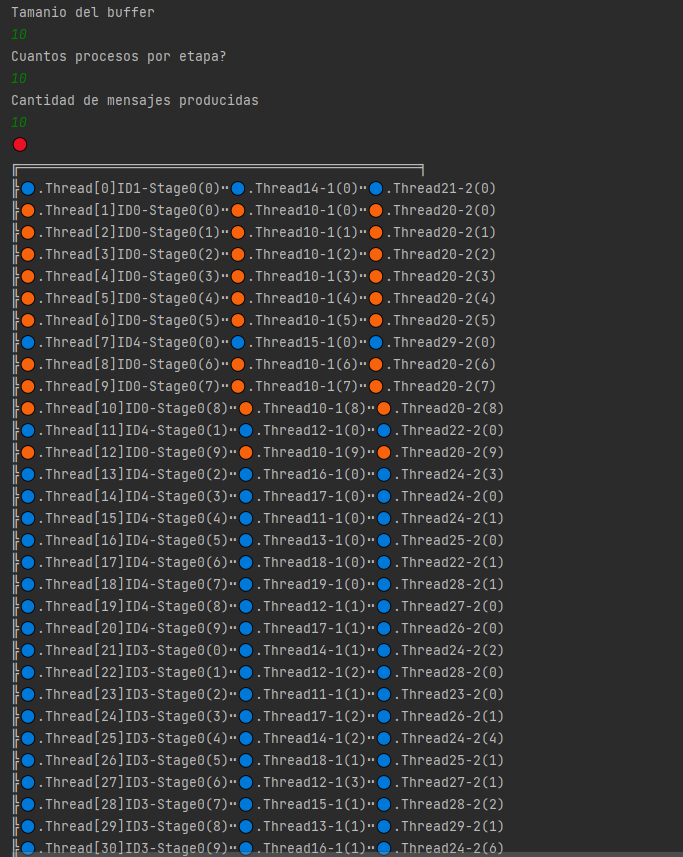
\includegraphics{10-10-10.PNG}

\subsubsection{3-3-3}
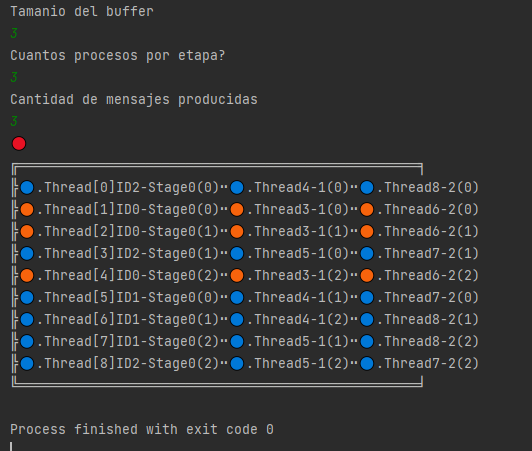
\includegraphics{3-3-3.PNG}

\subsubsection{5-5-5}
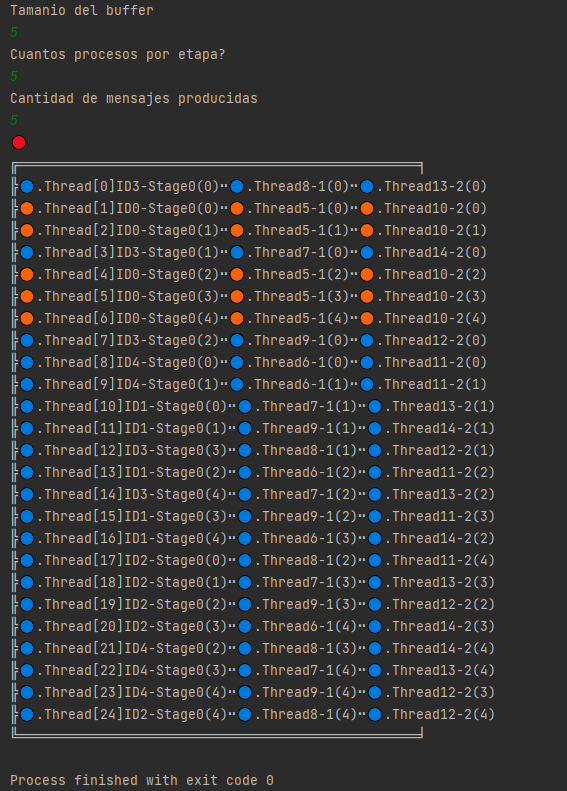
\includegraphics{5-5-5.PNG}

\section{Glosario}
\paragraph{Función Lambda}

\paragraph{Objeto anónimo}


%------------------------------------------------
\end{document}
